% IMPORTANT: PLEASE USE XeLaTeX FOR TYPESETTING
\documentclass[10pt]{beamer}

\usetheme{Darmstadt}%{default}
\usecolortheme{beaver}
\usepackage[T1]{fontenc} 
\usepackage[utf8]{inputenc}
\usepackage[french]{babel}
\usefonttheme{serif}
\usepackage{lmodern}
\usepackage{tcolorbox}
 % pour un pdf lisible à l'écran
 % il y a d'autres choix possibles 
\usepackage{pslatex}
% \usepackage{ctex, hyperref}
\usepackage{latexsym,amsmath,xcolor,multicol,booktabs,calligra}
\usepackage{graphicx,pstricks,listings,stackengine}
\usepackage{chemfig}

\usepackage{tabularx}
% meta-data

\author{Gabriel Le Doudic}
\institute{Préparation à l'agrégation de Rennes}
% \titlebackground{images/background}

\definecolor{aquamarine}{rgb}{0.5, 1.0, 0.83}
\definecolor{applegreen}{rgb}{0.55, 0.71, 0.0}	
\definecolor{cobalt}{rgb}{0.0, 0.28, 0.67}

\definecolor{definitionf}{RGB}{220,252,220}
\definecolor{definitionl}{RGB}{39,123,69}
\definecolor{definitiono}{RGB}{72,148,101}

\definecolor{propositionf}{RGB}{255,216,218}
\definecolor{propositionl}{RGB}{38,38,38}
\definecolor{propositiono}{RGB}{109,109,109}

\definecolor{theof}{RGB}{255,216,218}
\definecolor{theol}{RGB}{160,0,4}
\definecolor{theoo}{RGB}{221,65,100}

\definecolor{avertl}{RGB}{163,92,0}
\definecolor{averto}{RGB}{255,144,0}

\definecolor{histf}{RGB}{241,238,193}

\definecolor{metf}{RGB}{220,230,240}
\definecolor{metl}{RGB}{56,110,165}
\definecolor{meto}{RGB}{109,109,109}


\definecolor{remf}{RGB}{230,240,250}
\definecolor{remo}{RGB}{150,150,150}

\definecolor{exef}{RGB}{240,240,240}

\definecolor{protf}{RGB}{247,228,255}
\definecolor{protl}{RGB}{105,0,203}
\definecolor{proto}{RGB}{174,88,255}

\definecolor{grid}{RGB}{180,180,180}

\definecolor{titref}{RGB}{230,230,230}

\definecolor{vert}{RGB}{23,200,23}

\definecolor{violet}{RGB}{180,0,200}

\definecolor{copper}{RGB}{217, 144, 88}
%% CADRES

\newtcolorbox{defi}[1]{
	colback=applegreen!5!white,
  	colframe=applegreen!65!black,
	fonttitle=\bfseries,
  	title={#1}}
\newtcolorbox{Programme}[1]{
	colback=cobalt!5!white,
  	colframe=cobalt!65!black,
	fonttitle=\bfseries,
  	title={#1}}  
\newtcolorbox{Resultat}[1]{
	colback=theof,%!5!white,
	colframe=theoo!85!black,
  fonttitle=\bfseries,
	title={#1}} 
\usepackage{tikz}
\usepackage{array}
\usepackage[scientific-notation=true]{siunitx}
\usetikzlibrary{matrix}
\newcommand{\diff}{\mathrm{d}}

\title{Leçon : Notion de viscosité d'un fluide, écoulement visqueux}

% document body
\begin{document}
\begin{frame}{}
    \titlepage

    \begin{tabularx}{\textwidth}{l@{:\,\,}X}
        \textbf{Niveau} 	  & CPGE\\
        \textbf{Prérequis} & Hydrostatique\\
        &			Cinématique des fluides\\
        & 			Mécanique
    \end{tabularx}
\end{frame}

\begin{frame}
    \tableofcontents
\end{frame}
\section{Notion de viscosité}
\subsection{Contrainte visqueuse}
\subsection{Ordres de grandeur ($T=20^\circ~\rm C$)}
\begin{frame}
    \begin{table}
        \centering
        \resizebox{\columnwidth}{!}{
    \begin{tabular}{|c|c|c|}
        \hline
        &Viscosité dynamique $\eta$ (Pa$\cdot$s)& Viscosité cinématique $\nu=\eta/\rho$ ($\rm m^2\cdot s^{-1}$ et $P = 1$ bar) \\ \hline
        
        Eau & \num{e-3}& \num{1.006e-6} \\ \hline
        Air & \num{18.2e-6}&\num{15.1e-6} \\ \hline
        Glycérine & 1.49 & \num{11180e-6} \\ \hline
        mercure & \num{1.55e-3} & \num{0.116e-6} \\ \hline
        H2 & \num{8.83e-6} & \num{105e-6} \\ \hline
    \end{tabular}}
    \caption{Cours de Marc Rabaud \url{http://www.fast.u-psud.fr/~rabaud/NotesCours_Agreg.pdf}}
\end{table}
\end{frame}

\section{Exemple de l'écoulement de Poiseuille}
\subsection{Champ de vitesse de l'écoulement de Poiseuille}

\begin{frame}{\insertsubsection}
    \begin{figure}
        \centering
        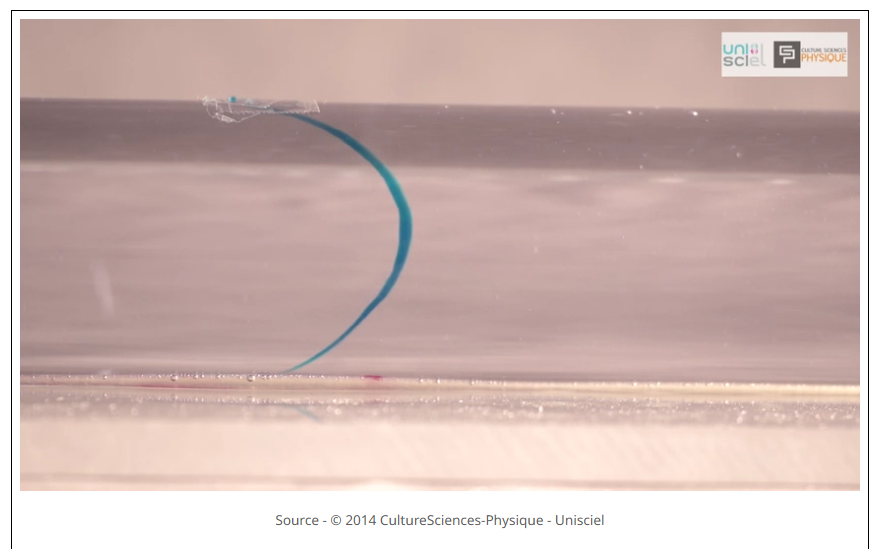
\includegraphics[width=.7\textwidth]{Poiseuille_ens_lyon.png}
        \caption{\url{https://culturesciencesphysique.ens-lyon.fr/ressource/physique-animee-poiseuille.xml}}
    \end{figure}
\end{frame}

\subsection{Mesure de la viscosité}
\subsection{Dissipation de l'énergie}
\subsection{Différents régimes d'écoulement (laminaire / turbulents)}
\begin{frame}{\insertsubsection}
    \begin{figure}
        \centering
        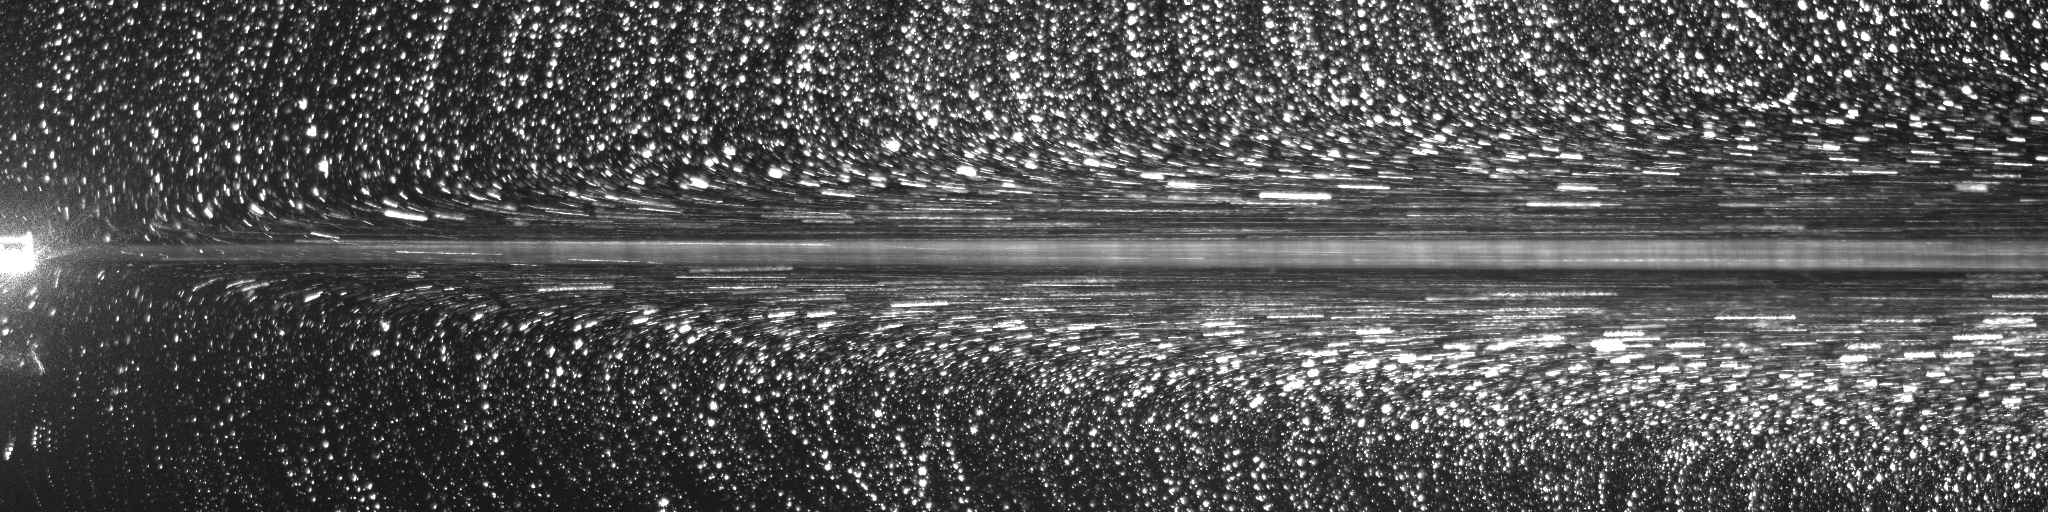
\includegraphics[width=.7\textwidth]{laminaire_Q75p63_texposure2ms_fps100.png}
        \caption{écoulement laminaire: $v = 14~\rm m\cdot s^{-1}$, $d =337~\rm \mu m $, $Re = 314$}
    \end{figure}
    \begin{figure}
        \centering
        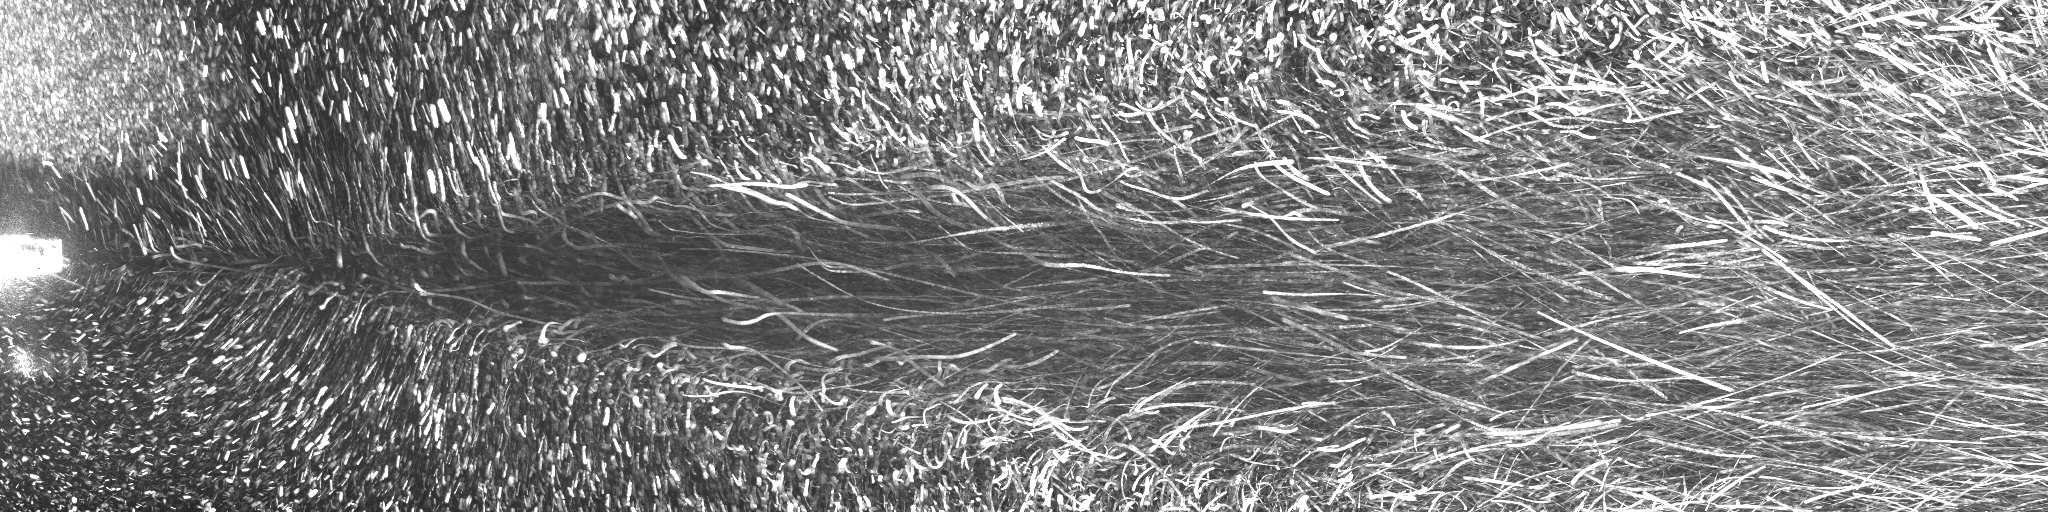
\includegraphics[width=.7\textwidth]{turbulent_Q157p87_texposure2ms_fps100_fumee_2_40images.png}
        \caption{écoulement turbulent: $v = 29~\rm m\cdot s^{-1}$, $d =337~\rm \mu m$, $Re = 652$}
    \end{figure}
\end{frame}
\end{document}